\chapter{Implementation}\label{chapter:implementation}
For this paper, we are implementing app prototypes to demonstrate the capability of pattern recognition as personal authentication factor. We chose Android as the main smart device platform, since access to development tools and documentation is freely available. Also Android applications are developed using Java, which allows to use many existing libraries. Android code also remains portable across different form factors of devices, such as phones, tablets and smartwatches running Android-Wear.

The development and testing of the Android application was conducted on the author's personal devices, an OnePlus One and a Nexus 10. To be able to develop an Android Wear app, the Chair of Operating Systems kindly provided a Sony Smartwatch 3.

For the implementation we also used SQL to store data gathered in tests platform-independently. To visualize and plot the sensor measurements and their correlation to keystrokes, we used Python with the excellent \emph{matplotlib}.

\section{Platform identification: Device vs.\ Server}
One of the first tasks when designing applications, is to analyze the target platform, the application should run on. For an authentication scenario, we can identify two different platforms: A client, in our case an Android device, and a server, which wants to authenticate a user. For our approach, we can use both platforms, to base the pattern recognition of the acceleration data on. Thus we can gather arguments pro and contra each platform.

We could process all the data locally on the device, since we already need an Android App to record the accelerometer data. When we do the data processing client-side, we can keep the server application as small as possible. Since typical Android devices have multi-core processors, they also should be computationally powerful enough to process the data. In our test scope, all sensor processing work was handled fast enough to not create any user noticeable wait times. Moreover, decentralized data processing on the individual devices also has significant advantages in reducing server load, which allows the authentication approach to easily scale to a big number of users.

Local processing of the acceleration data also reduces the size of the data transmitted to the server. The raw data can easily reach several megabytes, which is especially troublesome for mobile devices. When the networking connectivity of mobile devices can be slow, e.g.\ in cellular networks, raw data transmission can take several seconds.

There are also approaches to privacy protecting biometric authentication by locally generating cryptographic bio-keys\cite{bhargav2006privacy, verbitskiy2003reliable, ross2011visual}. Since handling personal identification information requires special precautions to not loose the data, these bio-keys can be used to implement so called ``zero-knowledge proof of knowledge'' protocols. This is especially useful, since only the information needed to verify the proof of knowledge needs to be stored on the server. If an attacker acquires this information, he can only verify the identity of the user and is not able to extract personal data about the user, thus preserving the users privacy.

A client-side data processing can also be used to authenticate the user locally, e.g.\ when entering the phones unlock code. This can be used for intrusion detection or for locking stolen devices.

However, server side authentication is easier to deploy, since changes in the authentication algorithms only need to be made in a single place. Authentication spoofing also is harder, since an attacker can analyze locally installed apps, but does not have access to the server application.

For this paper, we implemented a client-side authentication mechanism. In our opinion, the privacy of a user is very important and personal data should not be transmitted over the network, when it can be avoided.

\section{General purpose Android acceleration pattern detection library}
Since we are creating two different apps, a normal Android and an Android Wear variant, we quickly decided to share code among those apps. To do this, we created a general purpose acceleration pattern detection library for Android. This also allows rapid prototyping of the different approaches outlined in Chapter~\ref{chapter:approaches}.

The main goal of this library is easy integration into existing apps to enhance the authentication security without the need for specially crafted implementations. With our library, apps can compose their own pattern recognition implementations in a modular way, based on a stable and modular basis.

pipeline erklären
TODO: hier pipeline schaubild einfügen.


\subsection{Sensor recording in Android}\label{subsection:sensorrecording}
In Android, the access to sensors of the device is managed by the \lstinline$SensorManager$ class. The process of obtaining the \lstinline$SensorManager$, getting the default acceleration sensor and registering a custom \lstinline$SensorEventListener myListener$ is shown in Listing~\ref{lst:sensormanager}. The mechanic of getting data is then defined in the \lstinline$SensorEventListener$, which is periodically called by the Android system with new data.

\begin{lstlisting}[float,
caption={Obtaining the default acceleration sensor data in Android},
label={lst:sensormanager}]
SensorManager mgr = (SensorManager) context
    .getSystemService(Context.SENSOR_SERVICE);
Sensor sensor = (manager.getDefaultSensor(Sensor.TYPE_ACCELEROMETER));
mgr.registerListener(myListener, sensor, SensorManager.SENSOR_DELAY_FASTEST);
\end{lstlisting}

The rate at which the \lstinline$SensorEventListener$ gets callbacks is defined via the third parameter of the \lstinline$SensorManager.registerListener()$ function. In our case, we are using the fastest rate possible, since we don't want to miss even the slightest features of the movement pattern. Miluzzo et al.\cite{miluzzo2012tapprints} also have shown in their paper about guessing letters from device movement, that their results drastically improve with higher sensor sampling rate. Hence, we chose to simply poll the sensor at the fastest rate possible, with \lstinline$SensorManager.SENSOR_DELAY_FASTEST$. In our tests, this corresponds to a sapling rate of about $\SI{200}{\hertz}$.

\subsection{Sensor measurement framework}
Within the library, we provide a simple way to record sensor values into a predefined data structure, called \lstinline$SensorData$. All classes defined to measure and record the sensors are organized in the \lstinline$measurement$ package.

The \lstinline$SensorData$, as shown in Listing~\ref{lst:sensordata}, consists of a two-dimensional array of floats, called \lstinline$data$. The first dimension of this defines the direction of the sensor measurement, i.e.\ X- Y- and Z-acceleration, while the second dimension defines the series of individual measurements. We also record a timestamp of the individual measurements in the \lstinline$timestamps$ array. This is necessary, since the time between measurements can vary, depending on the current load of the processor.
For example, if we access \lstinline$data[0][41]$, we get the \nth{42} measurement of the X-acceleration in the series. The corresponding timestamp can be accessed via \lstinline$timestamps[41]$.

\begin{lstlisting}[float,
caption={Class \lstinline$SensorData$ containing the raw sensor readings},
label={lst:sensordata}]
public class SensorData {
    
    public final float[][] data;
    public final long   [] timestamps;

    public SensorData(float[][] data, long[] timestamps) {
        this.data = data;
        this.timestamps = timestamps;
    }

    public int getDimension() {
        return data.length;
    }
}
\end{lstlisting}

Since arrays with static size are not suitable for building up data, we also defined a corresponding \lstinline$SensorDataBuilder$, that uses lists of dynamic size to append new measurements. We can do this by calling the instance method \lstinline$SensorDataBuilder.append()$, that dynamically grows the list as needed. When we completed recording of new measurements, we can create a \lstinline$SensorData$ object of these measurements with the \lstinline$SensorDataBuilder.toSensorData()$ method.

The reasoning behind converting the data from lists to arrays, is that arrays have significantly less overhead, in accessing random data as well as memory consumption. Also the preprocessing and feature extraction steps usually operate on simple arrays. So instead of converting the data for each step, we only use dynamic lists for buildup and use simple arrays afterwards.

\subsection{Preprocessing of SensorData}
To create meaningful and comparable sensormeasurements, we needed to implement a preprocessing step after recording the sensor data. Since the measured acceleration includes gravity, we need to factor it out, depending on how the user holds the device.

To negate the effect gravity has on the measured data, we assume, that the device is relatively static in overall acceleration. This holds true for most applications, such as the device is lying on a desk or a user is carrying it around. We neglect the fact, that we cannot simply factor out gravity when we are measuring in a changing acceleration environment, e.g. driving in a car.

To factor out the gravity, we normalize the measured data to get a mean value of 0. We can do this by simply calculating the mean value and shift all sensor values by the negative mean, which results in the mean afterwards being 0. This results in an overall formula of: $ x_{new} = x - \mu $ with $\mu$ being the mean of the measurement.

To enhance the sensor recordings, we also implemented smoothing functions, that are able to dampen sensor noise. As for this paper, we implemented a simple moving average and exponential smoothing filters. The simple moving average algorithm works by averaging a certain number of measurements in a so called ``window size''. For comparison, we also implemented a simple moving average filter, which factors in the last smoothed value with a factor $\alpha$ with $0 < \alpha < 1$.

TODO: normal signal vs. moving average vs. exponential figure.

Since the rate of sensor measurements can vary with the processor load, we also could interpolate the measurements to a continuous function or simply a fixed rate. A technique to implement this would for example be cubic spline interpolation. However our sensor measurements are fairly regular and sufficient for a proof-of-concept, with a standard variance in measurements $< 0.01ms$. In real world applications with varying loads and background activity during sensor measurements, this might be needed.

Since there might be multiple preprocessing steps needed, we also implemented a simple \lstinline$ComposingPreprocessor$, which can combine multiple preprocessing steps to a single one. We then simply apply the other preprocessors sequentially as specified. Thus we can for example first noremalize the data to a mean of 0 and then smooth it with one of the implemented smoothing functions.

\subsection{Feature extraction from SensorData}\label{subsection:featureextraction}
test

Transformation into FeatureVectors
PeakDetector

PhoneKeystrokeFeatureExtractor -> Tap intensity and dwell time
Parameters for peak detection

WearKeystrokeFeatureExtractor -> Tap intensity, dwell time and wear movement

\subsection{Classification and machine learning}

distance between feature vectors via DTW classification
clustering and classification with kNN Classifier, implement Encog?

\section{Data storage and processing}
Persistent storage is important -> machine learning
Replay of previously recorded data to compare approches

\subsection{SQLite Database}
SQLite lightweight database. standard android. no need for extra features

.db file can be easily shared among devices -> data visualization via python
\begin{figure}
    \centering
    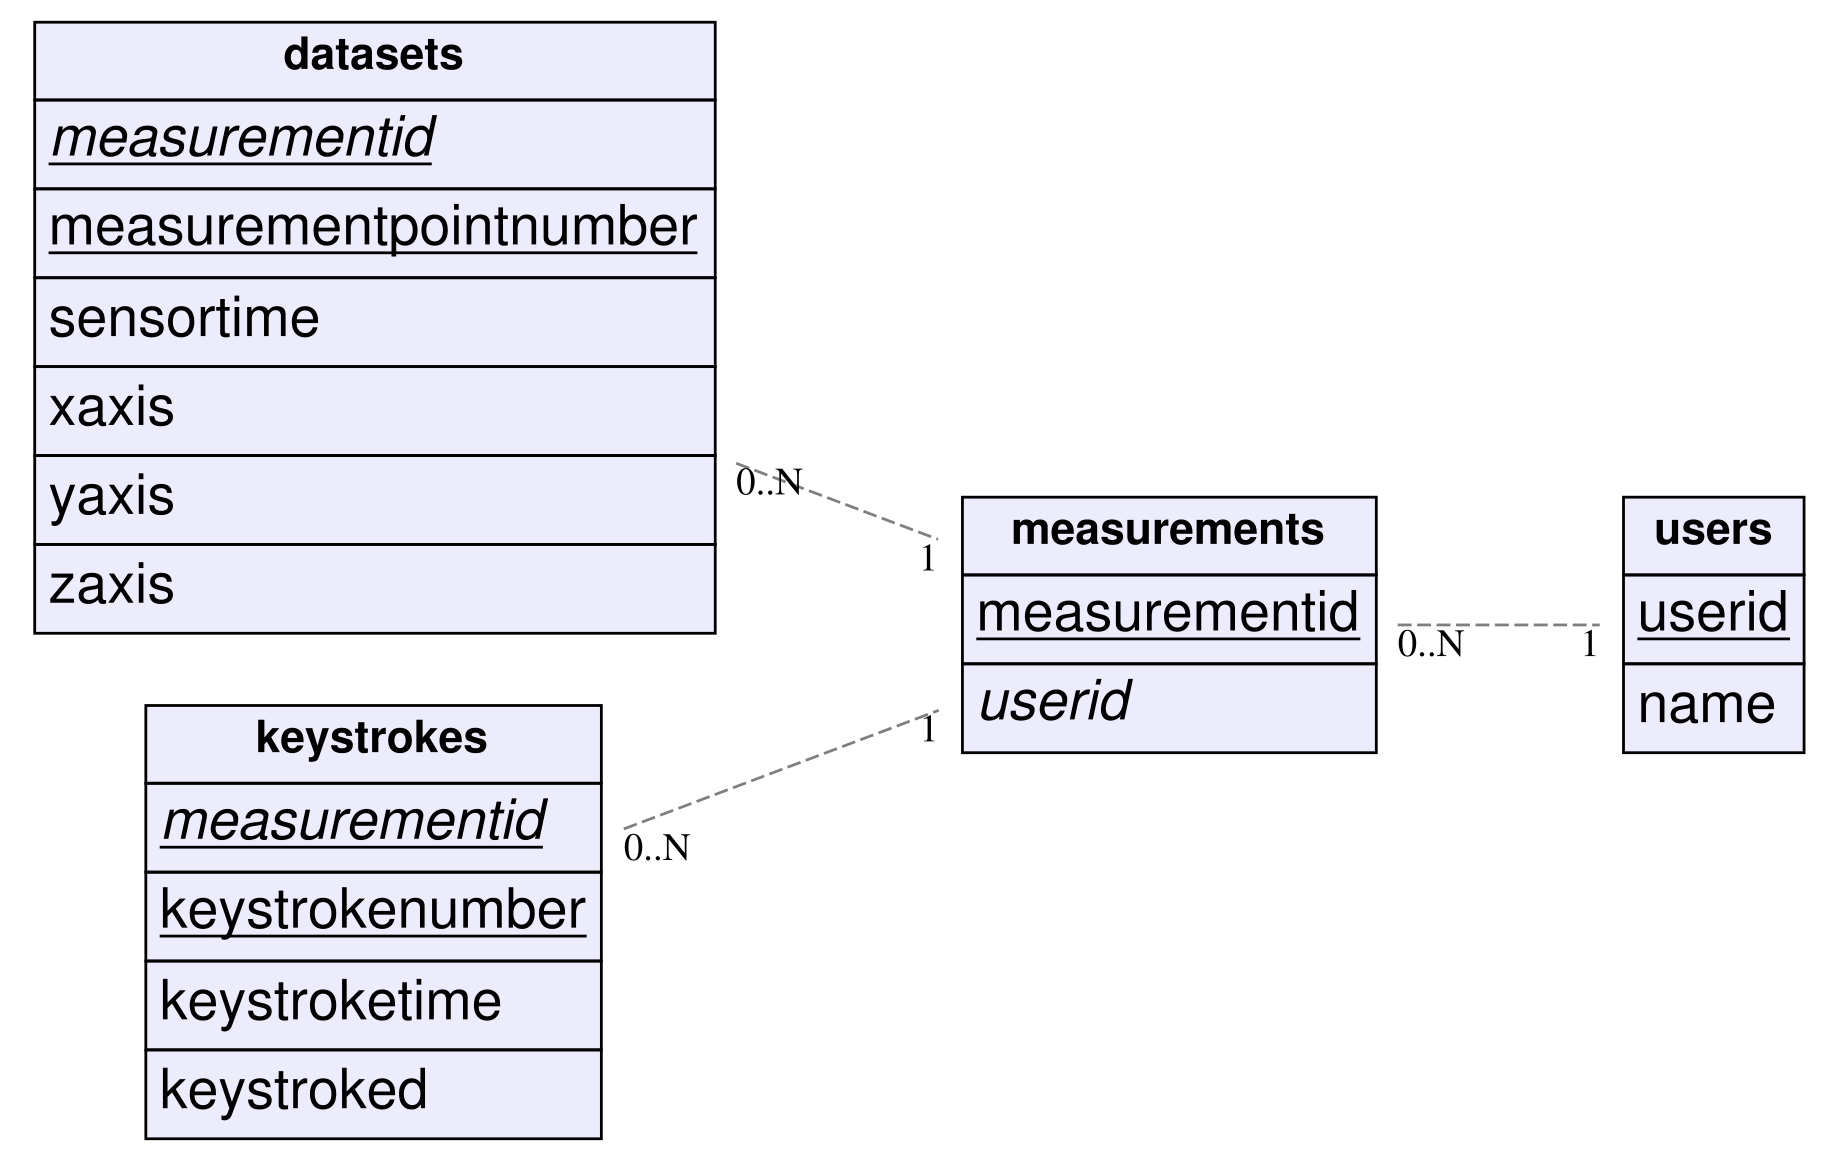
\includegraphics[width=\textwidth]{figures/databaseschema.png}
    \caption{Schema of the SQLite database used by the prototypes}
    \label{fig:dbschema}
\end{figure}

\subsection{Background verification of patterns}
Planned enhancement for unobstructed user experience. Not implemented yet

\section{App prototypes}
App prototypes on Github. Android Studio project, 3 different modules to share code between Phone and Wear project

Sensorprocessing: Implementation of the sensor recording, preprocessing, analyzing and classification

App: Phone / Standard Android module, Activities for Text input / user information what this app does

Right now: only proof of concept, due to limited time. No real authentication of users. demonstrating 

TODO: figure of module structure

\subsection{Android application}
TODO: application screenshots

onFocusChangeListener to define start and end of text input

combined authenticator: accelerometer, normalizer, smoothing, PhoneKeystrokeFeatureExtractor, kNN Classifier with DTW distance

\subsection{Android Wear application}
TODO: wear screenshots



\subsection{Limitations}